\chapter{Développement d'une méthode d'imagerie cardio-vaculaire sang blanc 3D grâce à une séquence à temps d'écho ultra-court et l'injection d'un agent de contraste à base de nanoparticule de fer.}

\section{Contexte}

L'IRM est devenu un outil de référence pour l'imagerie cardio-vasculaire car elle peut permettre d'obtenir de manière non-invasive des informations anatomiques mais aussi fonctionnelle sur le coeur. L'imagerie résolue dans le temps du coeur 2D s'est donc fortement développée que ce soit chez l'homme ou le petit animal. 
Cependant celles-ci ne permettent pas d'obtenir une résolution importante dans la direction de coupe et peuvent sous-estimer des défauts de contraction du myocarde ou donner des informations sur la fraction d'éjection peu précise, en particulier pour des cas pathologiques entrainant des modification de la paroi du myocarde \cite{Friedrich:2000aa}.
Le passage à l'imagerie 3D pour des applications cardiovasculaire a donc un intérêt considérable. Cependant, celui-ci s'est confronté au faible CNR entre le sang et le myocarde provoqué à la saturation des spins avec les séquences traditionnelles d'imagerie cardiaque de type écho de gradient. 
De nouvelles stratégies ont été employé pour obtenir un bon SNR et CNR sur les images comme l'utilisation de séquence de type "Balanced Steady-State Free Precession" (BSSFP) qui permettent d'obtenir un meilleur signal des liquides et donc du sang \cite{Nezafat2008Inflow-quantifi}. Cependant cette méthode est sensible aux variations local de champs magnétique ce qui a pour effet de créer des artéfacts caractéristiques sous forme de bande noire. Cela explique sa faible utilisation pour des applications à haut-champ magnétique et en particulier sur le petit animal. Des méthodes de correction de ces artéfacts ont été développées par Miraux et al. mais requiert un temps d'acquisition 4 fois plus long \cite{Miraux:2008sf}. Une autre approche possible et l'utilisation de séquence sang noir qui permettent d'obtenir des mesures plus précises de l'anatomie cardiaque \cite{Berr2005Black-blood-gra} mais cela au détriment du SNR des images ce qui nécessite ici aussi d'augmenter le temps d'accumulation des images \cite{Miraux:2009rm}.
En pratique clinique, l'injection d'agents de contraste à base de gadolinium peut être utilisé pour l'imagerie cardiaque résolue dans le temps mais n'est pas adapté pour des applications précliniques. En effet l'agent de contraste est excrété rapidement ce qui est particulièrement limitant pour des applications cardiovasculaire chez le petit animal nécessitant des temps d'acquisitions plus long. De plus le gadolinium, de par son faible poids moléculaire, diffuse facilement dans le compartiment interstitiel ce qui a pour effet de réhausser le signal dans le myocarde et donc de diminuer le contraste avec le sang.

L'utilisation d'agents de contraste à base de nanoparticules de fer (USPIO) en tant qu'agent de contraste positif restreint au système vasculaire semble être une bonne alternative aux agents à base de gadolinium grâce à leurs temps de vie dans le sang élevé  \cite{Corot:2006fk,Neuwelt:2009aa}.
Il a déjà été montré que ce type d'agent de contraste pouvait être utilisé à des champs magnétiques cliniques (1,5T et 3T) pour l'imagerie de premier passage \cite{Li:2005uq}, pour l'imagerie vasculaire \cite{Sigovan:2009aa,Nayak:2014aa} ainsi que pour l'imagerie cardiaque \cite{Amano:2000aa}.
Sur le petit animal, la plupart des études utilisant des USPIOs ont été réalisées à des champs inférieurs ou égaux à 3T (\cite{Jung:2014aa,Girard:2011ec,Loubeyre:1997aa}. Cependant la plupart des IRM pré-cliniques disponibles utilisent des champs magnétiques supérieurs à 4,7T. Hors, à hauts champs magnétiques l'effet $T_2^*$ provoqué par les USPIOs est plus important alors que l'effet $T_1$ est pratiquement stable. Cela explique pourquoi les USPIOs sont principalement utilisés en tant qu'agents de contraste négatif. Mais ceux-ci peuvent tout de même être utilisé en tant qu'agents de contrastes positifs en limitant leurs effet $T_2^*$. Pour cela il est nécessaire de limiter la décroissance du signal causé par le déphasage des spins autour des USPIOs et, à ce jour, la meilleur méthode disponible et de réduire fortement les temps d'échos des séquences utilisées.
Récemment, Gharagouzloo et al. \cite{Gharagouzloo:2014aa} ont réussi a obtenir un contraste positif de tout le système cardio-vasculaire à 7 Tesla après l'injection de Ferumoxytol\textregistered \ en utilisant une séquence radiale à temps d'écho ultracourt (UTE).

Dans ce chapitre je montrerai qu'en combinant l'utilisation d'une séquence 3D UTE (TE < 0.050 ms) et l'injection d'USPIO il est possible d'obtenir un contraste positif à différentes valeurs de hauts champs magnétique (4,7T, 7T et 9,4T) ainsi qu'avec un large panel de concentration d'USPIO injecté. A partir de ce principe je montrerai qu'il est possible, grâce à un schéma d'acquisition original, d'obtenir à partir d'un même jeu de donnée acquis des images en 3D résolue dans le temps de tout le système cardio-vasculaire avec une forte résolution spatiale ainsi que des images avec une forte résolution temporelle.

\section{Angiographie rehaussé par un agent de contraste à base de nanoparticules de fer}

\subsection{Agent de contraste}

Les agents de contrastes à base de particules de fer sont séparées en plusieurs catégories en fonction de leurs tailles. Les USPIOs ont une taille inférieur à 50 nm. Ils sont composées d'un noyau cristallin d'oxyde de fer entouré d'un "coating" (enrobage généralement composé de dextran) qui évite leur agrégation dans l'organisme. Les USPIOs sont généralement captés par le foie et la rate après une injection par voie intraveineuse. Une des propriétés qui est intéressante pour l'imagerie cardiaque est leurs longues durées de vie plasmatique (supérieur à 36 heures).

Durant ce projet nous avons utilisé plusieurs USPIOs différents : 
\begin{enumerate}
\item Le Sinerem \textregistered \ (Guerbet, France) : C'est un dérivé du ferumoxtran-10, il possède un petit diamètre hémodynamique (30 nm) et un long temps de rémanence vasculaire. Celui-ci est extrêmement espèce dépendant (Demi-vie plasmatique chez l'homme : 36 heures, chez le lapin 6 heure, chez le rat : 2 heures). Le ferumoxtran-10 est complétement dégradé dans les lyposomes des macrophages en sept jours. Celui-ci a été autorisé sur le marché européen pour la détection des métastases des ganglions lymphatiques.

\item Le P904 (Guerbet, France) : C'est un agent de contraste prototype préclinique mis en place pour l'imagerie des macrophages, l'imagerie cellulaire ou l'angiographie. Sa demi-vie plasmatique est également espèce dépendante (Chez la souris : 60 minutes, chez le rat : 145 minutes).
\end{enumerate}

Les relaxivités $r_1$ et $r_2$ de ces deux agents de contrastes ont des comportements équivalents en fonction du champs magnétique. Avec l'augmentation de celui-ci, le $r_1$ reste quasi-constant et le $r_2$ va augmenter fortement. Les variations de relaxivité observées en fonction du champs peuvent limiter ou nécessiter d'adapter les méthodes d'imagerie pour obtenir un contraste positif. Les résultats présentées dans cette thèse ont été obtenues avec l'injection du Sinerem mais des résultats équivalents ont aussi été obtenue avec le P904.

\subsection{Contraste positif en fonction du champs magnétiques et de la concentration}

Pour évaluer l'effet de l'agent de contraste sur les images, deux séquences ont été comparées dans cette partie. Une séquence classique cartésienne FLASH avec un temps d'écho TE = 1,4 ms et une séquence 3D UTE (TE = 0,031 ms). Les deux séquences ont été appliquées sur des souris injectées avec 3 valeurs de concentration de Sinerem (100,200 et 500 $\mu$mol de fer/kg) pour obtenir des images sur une zone allant du foie au cou. Ces valeurs de concentration ont été choisies car elles correspondent à une gamme allant des valeurs utilisées pour l'injection chez l'humain aux valeurs de concentration utilisées pour le ciblage cellulaire.
Les paramètres des séquences ont été fixés pour obtenir une résolution de $(234\mu m)^3$ isotropique et pour un temps d'acquisition de 3 min 41 sec pour la séquence FLAHS et de 3 min 51 sec pour la séquence UTE.

\begin{figure}[H]
\centering
\line(1,0){400} \\
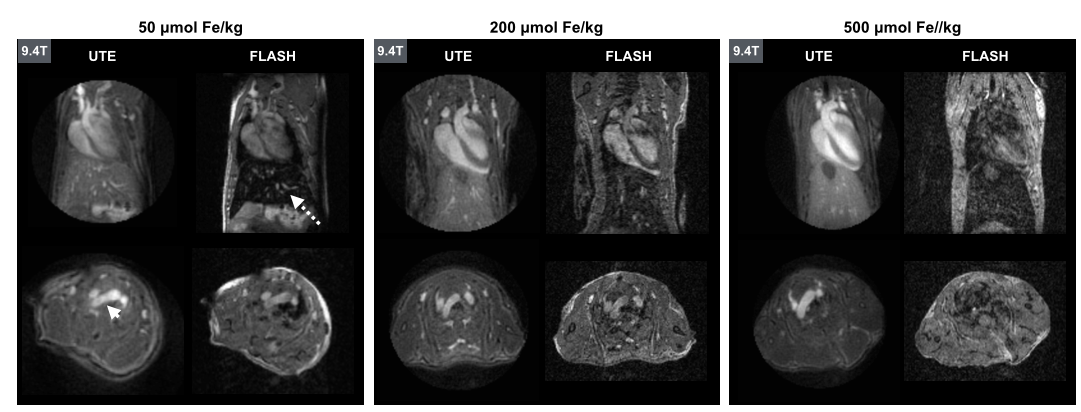
\includegraphics[scale=0.5]{./figure/chap4/UteVSFlash.png}
\caption[UTE vs Flash]{\label{fig:UteVSFlash} Images obtenues sur le coeur et le foie de souris avec une séquence 3D UTE et FLASH à 9,4T. Les images ont été obtenues pour différentes concentration de doses injectées (100,200 et 500 $\mu$mol Fe/kg), sans synchronisation cardiaque ou respiratoire.}
\line(1,0){400} \\ 
\end{figure}

Des images obtenues à 9,4 T avec les deux séquences sont montrées dans la figure \ref{fig:UteVSFlash}. Après l'injection de l'agent de contraste, le sang dans les vaisseaux est visible avec la séquence UTE avec un signal intense et ce quelque soit la dose injectée. Ce signal est très homogène même dans les zones avec de forte turbulence comme la crosse aortique indiqué par la flèche blanche ou dans les vaisseaux avec un faible débit comme les veines jugulaires. Avec la séquence FLASH, seul les deux plus faibles concentrations permettent de rehausser le signal du sang. Cependant cette augmentation du signal est faible et très hétérogène par rapport à la séquence UTE. Avec la plus forte concentration, le signal du sang a un signal plus faible que le signal des muscles environnant.

Des observations similaires ont été faite à 4,7 et 7T. Des valeurs de CNR ont été mesurées entre le sang (dans la crosse aortique et les veines jugulaires) et les muscles (figure \ref{fig:CNRUteFlash}). On observe qu'avec la séquence FLASH le signal décroit lorsque l'on augmente la concentration et devient même négatif avec la plus forte concentration alors qu'avec la séquence UTE on observe une augmentation considérable du CNR en fonction de la dose. Cette observation s'explique par l'effet $T_2^*$ qui augmente avec la concentration et qui a pour effet de diminuer le signal pour les séquences avec un TE long comme la séquence FLASH alors que la séquence UTE n'est pas impacté grâce à son TE ultracourt. Au contraire son signal augmente grâce à l'effet $T_1$ des USPIOs.
Le deuxième point à noter est que pour chaque concentration, que ce soit en UTE ou en FLASH, le signal diminue aussi avec l'augmentation du champs magnétique ce qui s'explique par la diminution des valeurs de relaxivité $r_1$ pour la séquence UTE et aussi par l'augmentation des valeurs de relaxivité $r_2$ pour la séquence FLASH.

\begin{figure}[H]
\centering
\line(1,0){400} \\
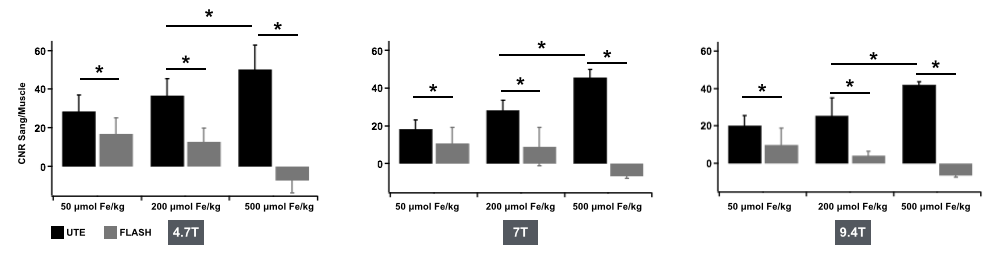
\includegraphics[scale=0.5]{./figure/chap4/CNRUteFlash.png}
\caption[CNR UTE vs Flash]{\label{fig:CNRUteFlash} Mesure du contraste sur bruit entre la crosse aortique et le muscle obtenue avec une séquence UTE et FLASH après injection d'USPIO à 4,7,7 et 9,4 T et pour différentes concentration de doses injectées (100,200 et 500 $\mu$mol Fe/kg). Les valeurs de p inférieures à 0,05 sont indiquées par des astérisques.}
\line(1,0){400} \\ 
\end{figure}

Quelque soit la concentration injectée les valeurs de CNR sont toujours supérieures avec la séquence UTE. De plus, peu d'artéfact de flux ou de mouvement sont observé avec la séquence UTE ce qui s'explique par la trajectoire radiale (voir la section \ref{subsec:MouvEtFlux}) ainsi que par le faible TE et l'absence de déphasage des spins par des gradients avant la lecture du signal.
Tous ces points font de la méthode d'imagerie combinant l'injection d'USPIO et l'utilisation d'une séquence UTE une stratégie envisageable pour l'angiographie 3D et en particulier l'imagerie cardiaque.

\section{Angiographie cardiaque 3D résolue dans le temps}

Au vue du très bon signal obtenue sur les images précédentes, il est envisageable de développer une séquence 3D résolue dans le temps. Cependant l'application de la méthode cinés à la séquence UTE nécessitent trop de temps d'acquisition si l'on souhaite obtenir des images respectant le critère de Nyquist. Par example pour des images avec une matrice $(128)^3$, il serait nécessaire de recueillir 102943 projection ce qui correspondrait à un temps d'acquisition de 257 minutes chez une souris avec un rythme cardiaque à 450 battement par minute. Heureusement, il est possible de sous-échantillonner l'acquisition d'un facteur 2 en impactant peu la résolution mais ce n'est pas suffisant pour une application en routine. Un autre point intéressant est que les séquences UTE disposent aussi d'un faible TR < 3.5 ms, il est possible de recueillir de nombreux signaux IRM (au moins 40) entre deux battement de coeur. Il est donc possible de regrouper des signaux ensemble pour diminuer le temps d'acquisition mais en limitant le nombre d'images résolues dans le temps qui seront reconstruites. 
Cependant cela nécessite de modifier la séquence pour que les signaux recueillies successivement ne suivent pas les mêmes trajectoires.


\subsection{Séquence}

J'ai donc développé une séquence UTE permettant d'obtenir un nombre d'image ciné (NCine) dont NRegroup signaux IRM recueillis successivement seront regroupé pour reconstruire une image. Dans nos expériences chez la souris les paramètres ont généralement été fixés à NCine = 10 et NRegroup = 4. Cela correspond donc à une acquisition de $10 \times 4 = 40$ signaux FIDs à recueillir entre deux battements. Ces paramètres peuvent être adaptés en fonction du rythme cardiaque de l'animal ainsi que du TR de la séquence. Avec des TRs de 2 ms pour une souris ayant un temps entre deux pics ECG de 140 ms, il est donc théoriquement possible de recueillir 70 signaux et de les regrouper par groupe de 7 pour accélérer la séquence d'un facteur 7 et reconstruire 10 images cinés.

\begin{figure}[H]
\centering
\line(1,0){400} \\
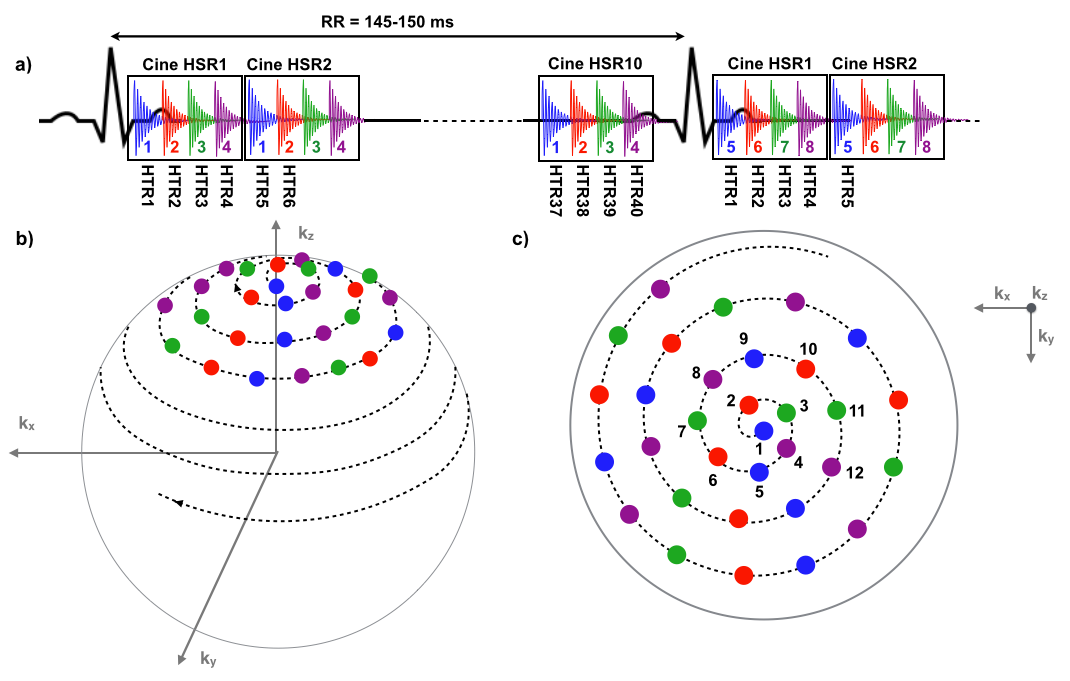
\includegraphics[scale=0.5]{./figure/chap4/SeqUTEUSPIO.png}
\caption[Séquence UTE USPIO]{\label{fig:SeqUTEUSPIO} Séquences d'acquisition de la séquence 3D UTE synchronisée sur le rythme cardiaque utilisée avec NCine = 10 et NRegroup = 4.}
\line(1,0){400} \\ 
\end{figure}

La séquence développée est présentée dans la figure \ref{fig:SeqUTEUSPIO} avec pour paramètres NCine = 10 et NRegroup = 4. La trajectoire utilisée pour positionner les projections est une spirale qui part en haut de l'axe Z et termine en bas en tournant autour de l'axe \cite{Saff1997}. La position des projections est définie par :
\begin{equation}
\begin{split}
	& For \ 1 \leq k \leq NPro : \\ 
	& h_k = -1+\frac{2(k-1)}{NPro-1} \\
	& \Theta_k = arcos(h_k) \\
	& \\
	& \Phi_1=\Phi_N=0 \\	
	& for \ 2 \leq k \leq N-1 \\
	& \Phi_k=\left( \Phi_{k-1}+\frac{3,6}{\sqrt{NPro\times (1-h_k^2)}} \right)mod(2 \pi)	
\end{split}
\end{equation}
où NPro correspond au nombre de projection utilisé pour parcourir un espace de Fourier. La méthode de répartition des trajectoires permet de les répartir de manière uniforme dans une sphère et ce quelque soit le nombre NPro défini. Cependant dans le cadre de cette séquence NPro doit être un multiple de NRegroup pour regrouper les projections ensemble pour former une image.

Les NRegroup = 4 premières projections sont recueillies selon des trajectoires différentes (1,2,3 et 4) comme montré sur la figure \ref{fig:SeqUTEUSPIO}.c. Ce schéma de trajectoire est répété NCine = 10 fois jusqu'au prochain battement de coeur où les 4 trajectoires utilisées sont alors celles numérotées (5,6,7 et 8).

\subsection{Reconstruction}

\begin{figure}[H]
\centering
\line(1,0){400} \\
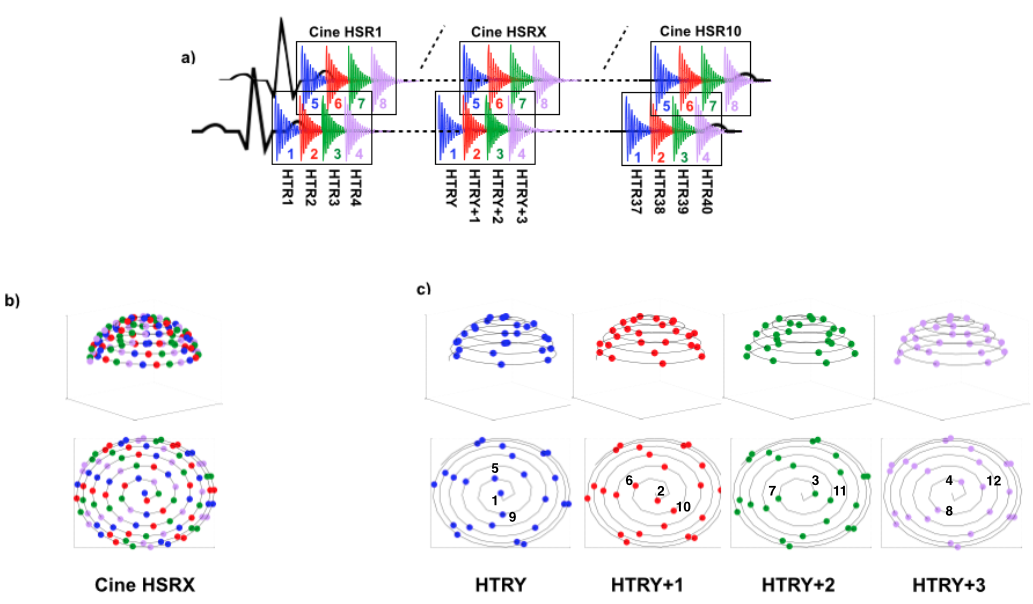
\includegraphics[scale=0.5]{./figure/chap4/RecoUTEUSPIO.png}
\caption[Reconstruction séquence UTE USPIO]{\label{fig:RecoUTEUSPIO} Représentation des projections utilisées pour reconstruire les jeux de données a) haute résolution spatiale et b) haute résolution temporelle.}
\line(1,0){400} \\ 
\end{figure}

Ce schéma d'acquisition permet de reconstruire à partir d'un même jeu de donnée acquis deux types d'images : NCine images avec une forte résolution spatiale (HRS) et NCine $\times$ NRegroup images avec une forte résolution temporelle (HTR). Pour reconstruire les images avec la forte résolution spatiale il faut utiliser toutes les projections recueillies durant la phase Cine HSRX (1245-5678-...) comme indiqué sur la figure \ref{fig:RecoUTEUSPIO}.a-b. L'espace de Fourier reconstruit est donc échantillonnée avec NPro projections.
Pour les images avec une forte résolution temporelle il faut séparer dans les projections recueillies dans la cine HSRX en 4 sous-partie correspondant aux couleurs que l'on reconstruira pour obtenir des images avec une meilleur résolution spatiale (NRegroup fois plus grande). Les images reconstruites auront une plus faible résolution spatiale car le nombre de projection sera NRegroup fois plus faible mais les projections seront réparties de manière pratiquement uniforme grâce à la trajectoire utilisée.

\subsection{Résultats}

\subsubsection{Angiographie résolue dans le temps à 4,7T, 7T et 9,4T.}

Des images 3D résolues dans le temps ont été recueillies avec une résolution de 156 $\mu$m isotropique pour les 3 champs magnétiques disponibles. La concentration intermédiaire de 200 $\mu$mol de Fe/kg a été injecté pour obtenir les images de la figure \ref{fig:UTEUSPIOField} mais des résultats similaires ont été observé avec la plus forte concentration. Ces images ont été obtenues avec pour paramètres : NCine = 10; NRegroup = 4; NPro = 18144; ce qui correspond à un temps d'acquisition d'environ 12 minutes.

\begin{figure}[H]
\centering
\line(1,0){400} \\
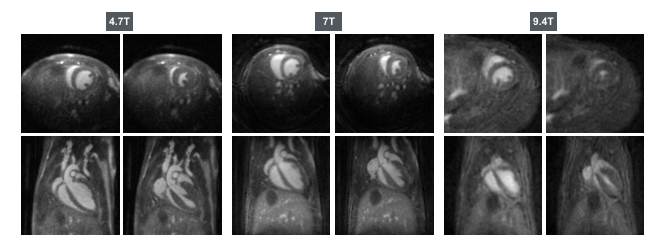
\includegraphics[scale=0.7]{./figure/chap4/UTEUSPIOField.png}
\caption[Images résolution 0,156 mm]{\label{fig:UTEUSPIOField} Image 3D obtenue sur un coeur de souris avec une résolution de 156 $\mu$m isotropique à différents champs magnétiques après l'injection d'USPIO à 200 $\mu$mol de Fe/kg. 10 images ont été reconstruites pour le cycle cardiaque, des images à la fin de la diastole (gauche) et de systole (droite) sont montrées dans deux orientations (En haut : petit axe; en bas : grand axe).}
\line(1,0){400} \\ 
\end{figure}

Des mesures de SNR et CNR ont été effectués dans le sang et le muscle du myocarde. On observe qu'un CNR d'environ 30 est obtenu dans le myocarde et le sang et ce quelque soit le phase du cycle cardiaque et le champs magnétique (voir les mesures de la figure \ref{fig:TableMidRes}). Le signal obtenu est très homogène dans les vaisseaux sanguins mais aussi dans les cavités du coeur : le signal mesuré sur des expériences à 7T montre que la déviation standard du SNR mesuré dans le sang des ventricules et la crosse aortique a une valeur comprise entre 1,4 et 2,2 pour un SNR de 70. La qualité des images obtenues à 4,7T et 7T est équivalente. Par contre à 9,4T les mesures de SNR/CNR sont plus faible ce qui s'explique par l'utilisation d'une antenne volumique de moins bonne qualité que les antennes surfaciques utilisées aux autres champs magnétiques.

\begin{figure}[H]
\centering
\line(1,0){400} \\
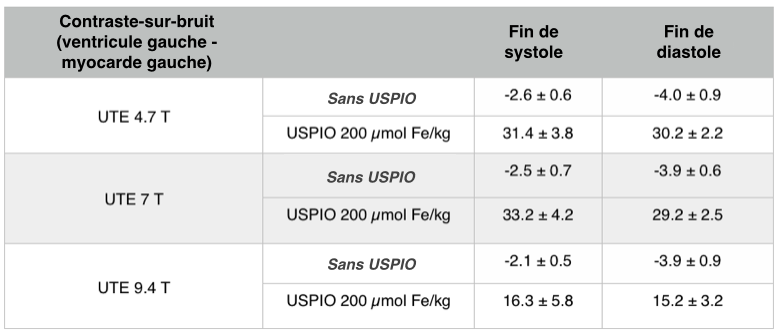
\includegraphics[scale=0.5]{./figure/chap4/TableMidRes.png}
\caption[Table SNR CNR Résolution moyenne]{\label{fig:TableMidRes} Mesure du CNR entre le sang dans le ventricule et la paroi du myocarde obtenue avec la séquence UTE avec une résolution de 156 $\mu$m isotropique à différents champs magnétiques après l'injection d'USPIO à 200 $\mu$mol de Fe/kg.}
\line(1,0){400} \\ 
\end{figure}

\subsubsection{Angiographie très-haute résolution.}

Des images ont été acquises avec une très forte résolution de 104 $\mu$m isotropique à 7T (figure \ref{fig:UTEUSPIOHRS}). Ces images ont été obtenues avec pour paramètre : NCine = 10; NRegroup = 4; NPro = 52540; ce qui correspond à un temps d'acquisition d'environ 35 minutes.
La concentration de l'agent de contraste injecté (200 $\mu$mol de Fe/kg) permet d'obtenir un très bon SNR dans le sang (40,2 $\pm$ 2,3) et d'un bon CNR entre le sang et le myocarde (15,8 $\pm$ 2,0) durant le temps de l'expérience.
Cette forte résolution nous permet d'obtenir des mesures de volumétrie précises qui sont en accord avec celles décrites dans la littérature. Mais surtout elle permet de parfaitement visualiser la déformation de la crosse aortique au cours du cycle cardiaque, de distinguer les valves aortique (Petit flèche, figure \ref{fig:UTEUSPIOHRS}.a) et de suivre les artères coronaires droite et gauche (flèches figure \ref{fig:UTEUSPIOHRS}.b).

\begin{figure}[H]
\centering
\line(1,0){400} \\
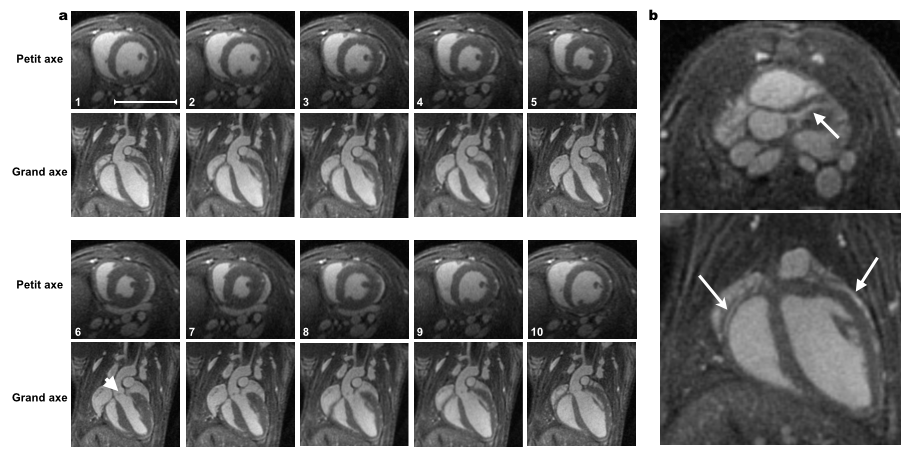
\includegraphics[scale=0.5]{./figure/chap4/UTEUSPIOHRS.png}
\caption[Image HRS]{\label{fig:UTEUSPIOHRS} a) Images 3D résolues dans le temps au cours du cycle cardiaque, obtenue à 7T avec une résolution isotropique de 104 $\mu$m après l'injection d'USPIO à 200 $\mu$mol de Fe/kg. Le petit axe est représenté dans la ligne du haut et le grand axe dans la ligne du dessous. La flèche (image 6) indique la valve aortique. b) Images extraites du volume 3D permettant de visualiser les artères coronaires. La barre d'échelle correspond à 1 cm.}
\line(1,0){400} \\ 
\end{figure}

A partir du même jeu de donnée il est aussi possible de reconstruire des images avec une forte résolution temporelle (figure \ref{fig:UTEUSPIOHRT}). Celles-ci permettent de visualiser la déformation du myocarde au cours du cycle cardiaque ce qui peut permettre d'étudier des modèles de trouble de la conduction cardiaque qui induiront un délai dans la contraction.

\begin{figure}[H]
\centering
\line(1,0){400} \\
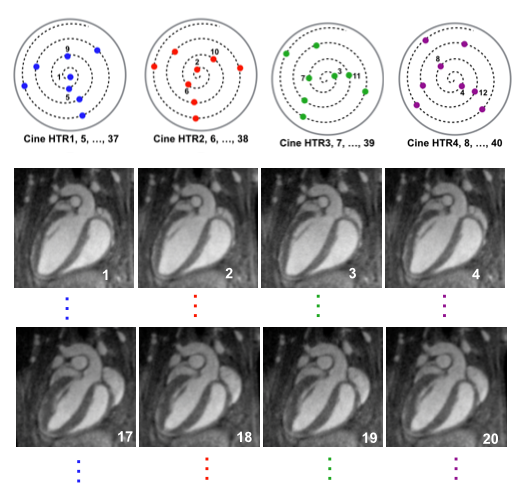
\includegraphics[scale=0.5]{./figure/chap4/UTEUSPIOHRT.png}
\caption[Image HRT]{\label{fig:UTEUSPIOHRT} a) Images 3D résolues dans le temps avec une forte résolution temporelle de 3,5 ms.}
\line(1,0){400} \\ 
\end{figure}

\section{Discussion}


Malgré ces nombreux avantages l'imagerie 3D chez la souris n'est toujours pas la méthode de référence pour étudier le coeur chez le petit animal. En effet la principale limitation est le faible SNR et CNR obtenus entre le sang et le myocarde. Dans cette optique, une nouvelle méthode d'angiographie cardiaque a été développée au cours de cette thèse permettant d'obtenir un contraste positif. 

Pour obtenir un contraste sang blanc en imagerie 3D dans ce projet, nous nous sommes orienté vers l'utilisation d'agents de contrastes à base de nanoparticules de fer car ceux-ci ont un effet $T_1$ qui permet de rehausser le signal du sang et ont une longue rémanence vasculaire. Une alternative possible est l'utilisation d'agent de contraste restreint au domaine vasculaire comme des liposomes chargés au gadolinium \cite{Ersoy:2004aa} mais ces agents n'ont pour le moment pas été approuvé pour des utilisations cliniques et leurs innocuités à long terme n'a pour le moment pas été validées. Au contraire, de nombreux agents à base de nanoparticules de fer ont déjà été validé pour des injections intraveineuse chez l'humain comme le Ferymoxytol/Feraheme ou bien le Sinerem. Leurs non-toxicités est donc un avantage pour des études longitudinales chez le petit animal.

Cependant les USPIOs n'avait jamais été utilisé à haut champs magnétique pour de l'angiographie sang blanc car le gain en signal devient de plus en plus faible avec l'augmentation du champs magnétique en utilisant les séquences cartésiennes. De plus, le choix de la dose devenait un problème car la gamme de concentration permettant de ne pas détériorer le signal est aussi de plus en plus restreinte. La solution développée dans ce travail a été l'utilisation d'une séquence radiale à temps d'écho ultracourt qui a permis de négliger l'effet de susceptibilité des nanoparticules. Grâce à cette séquence on observe, in vivo, une augmentation du signal en fonction de la concentration injectée d'agent de contraste et ce quelque soit le champs magnétique.

Cette méthode a été utilisé pour de l'imagerie 3D anatomique et résolue dans le temps sur le coeur de souris. Toutes les images montrent une très bonne homogénéité du signal et pas d'artéfact de mouvement ou de flux contrairement aux images 3D cartésiennes grâce à l'aspect radiale de la trajectoire UTE mais aussi à l'absence de gradient observé par les spins avant la lecture du signal. Cela permet une mesure extrêmement précise du volume des ventricules contrairement aux séquences d'imagerie sang blanc conventionnelles qui peuvent souffrir d'absence de signal particulièrement durant les phases systoliques du coeur. Le schéma d'acquisition original développé dans ce projet permet, à partir d'un même jeu de donnée, de reconstruire des images ayant une forte résolution spatiale et des images ayant une forte résolution temporelle qui permettent d'obtenir des informations fonctionnelles sur la contraction du myocardes au prix d'une plus faible résolution spatiale provoquée par le sous-échantillonnage des images. Cette méthode d'angiographie est aussi particulièrement adapté à l'imagerie de grand champs de vue situé au niveau du cerveau ou de l'abdomen (figure \ref{fig:UTEUSPIOAnat}) où les vitesses faibles des flux limites l'utilisation de séquence temps-de-vol. De plus, l'imagerie de la zone abdominal peut être particulièrement compliqué à cause de la respiration de l'animal ce qui renforce l'utilité de la séquence UTE pour sa robustesse au mouvement. 

\begin{figure}[H]
\centering
\line(1,0){400} \\
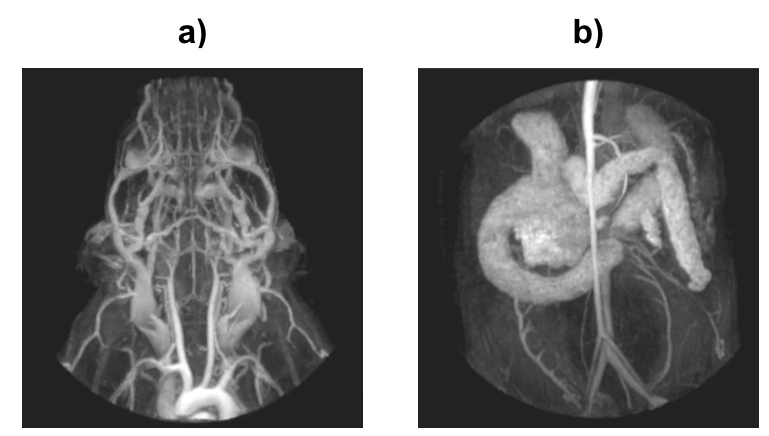
\includegraphics[scale=0.5]{./figure/chap4/UTEUSPIOAnat.png}
\caption[Imagerie anatomique UTE + USPIO]{\label{fig:UTEUSPIOAnat} Images anatomiques 3D d'une souris sur une zone : a) s'étendant de la crosse aortique au cerveau; b) abdominal.}
\line(1,0){400} \\ 
\end{figure}

La principale limitation de cette méthode d'acquisition est le fait que ce soit une séquence synchronisée sur le rythme cardiaque. La détection des pics ECG ne pose pas de problème car il y a très peu de changement des gradients d'imageries, par contre, il est nécessaire de stabiliser le rythme cardiaque de l'animal pour obtenir une image de bonne qualité. Cela peut être un problème pour les séquences permettant d'obtenir des images avec une très forte résolution spatiale car celles-ci peuvent durer plus de 35 minutes. Une solution est d'accélérer la séquence pour réduire la probabilité d'avoir des changements de rythme cardiaque importants. Les méthodes d'imagerie parallèle sont difficilement utilisable en pratique pré-clinique au vue du faible nombre de canaux des antennes, mais il a précédemment été montré que les séquences radiales sont favorables aux algorithmes de reconstruction de type "compressed sensing" qui peuvent limiter le temps d'acquisition \cite{Nam:2013nx}.
 
 
Cette méthode est a priori transposable chez l'homme bien qu'il faille l'adapter à d'autres contraintes. En effet, la séquence est ici seulement synchronisée sur le rythme cardiaque hors, chez l'humain, les mouvements respiratoires sont bien plus ample et doivent être corrigés.
Un deuxième point important est que la dose utilisée dans cette étude est supérieure à celle généralement injectée chez l'humain. En l'absence d'information supplémentaire il n'est pas possible aujourd'hui d'utiliser de tel concentration pour des injections en tant qu'agents de contraste. Cependant, des doses entre 50 et 100 $\mu$mol de Fe/kg combiné à la séquence 3D UTE devrait tout de même permettre d'obtenir, particulièrement à des champs $\leq$ 3T, des images du système vasculaire chez l'humain avec des résolutions temporelles et spatiales supérieures à celles obtenues pour le moment en pratique clinique. Le dernier point problématique à étudier est le temps d'acquisition important de cette séquence supérieur à 30 minutes, qui sera augmenté dans le cas d'une correction de la respiration. Celui-ci pourra être réduit d'au moins un facteur deux grâce à l'imagerie parallèle. De plus, les temps de répétitions utilisés dans cette étude sont de 3,5 ms. Cela est du aux limitations matérielles de nos imageurs mais il est cependant possible d'atteindre des TR inférieur à 2 ms avec les imageurs cliniques ce qui permettra de réduire le temps d'acquisition de la séquence de pratiquement un facteur 2. En combinant tous ces points on atteint des temps d'acquisitions égaux ou même inférieur à ceux obtenus pour le moment en routine clinique.









